\begin{tikzpicture}
\shorthandoff{>}
%
% Concavidad de - u log u
\begin{scope}[xscale=3,yscale=2.5]
\pgfmathsetmacro{\u}{.2};
\pgfmathsetmacro{\v}{1.25};
\pgfmathsetmacro{\l}{.7};
%
\draw[>=stealth,->] (-.5,0)--(1.6,0) node[right]{\small $t$};
\draw[>=stealth,->] (0,-.7)--(0,{1.5*log2(1.5)}) node[above]{\small $\phi(t) = t \log t$};
\draw[thick,domain=.005:1.5,samples=200] (0,0)-- plot (\x,{\x*log2(\x)});
\draw[dashed] (\u,{\u*log2(\u)})--(\v,{\v*log2(\v)});
\draw (\u,0)--(\u,-.05) node[below]{\small $t_1$};
\draw (\v,0)--(\v,-.05) node[below]{\small $t_2$};
%
\draw[dashed] ({\l*\u+(1-\l)*\v},.05) node[above]{\small $\pi_1 t_1 + \pi_2 t_2$}
--({\l*\u+(1-\l)*\v},{(\l*\u+(1-\l)*\v)*log2(\l*\u+(1-\l)*\v)});
%
% l phi(u) + (1-l) phi(v)
\draw[dotted]
({\l*\u+(1-\l)*\v},{\l*\u*log2(\u)+(1-\l)*\v*log2(\v)})--(-.05,{\l*\u*log2(\u)+(1-\l)*\v*log2(\v)})
node[left]{\small $\pi_1 \phi(t_1) + \pi_2 \phi(t_2)$};
%
% phi(l u + (1-l) v)
\draw[dotted]
({\l*\u+(1-\l)*\v},{(\l*\u+(1-\l)*\v)*log2(\l*\u+(1-\l)*\v)})--
(-.05,{(\l*\u+(1-\l)*\v)*log2(\l*\u+(1-\l)*\v)})
node[left]{\small $\phi(\pi_1 t_1 + \pi_2 t_2)$};
\end{scope}
%
%
% Concavidad / mezcla
\begin{scope}[xshift=8.5cm]
\draw(0,1.25) node{\includegraphics[width=3cm]{TIKZ_SZ/DosDados}};
\draw(-.5,2.5) node{\small $p_1$};
\draw(1,2) node{\small $p_2$};
\draw(2.7,1) node{\small $\pi_1 p_1 + \pi_2 p_2$};
\draw(-.25,-1) node{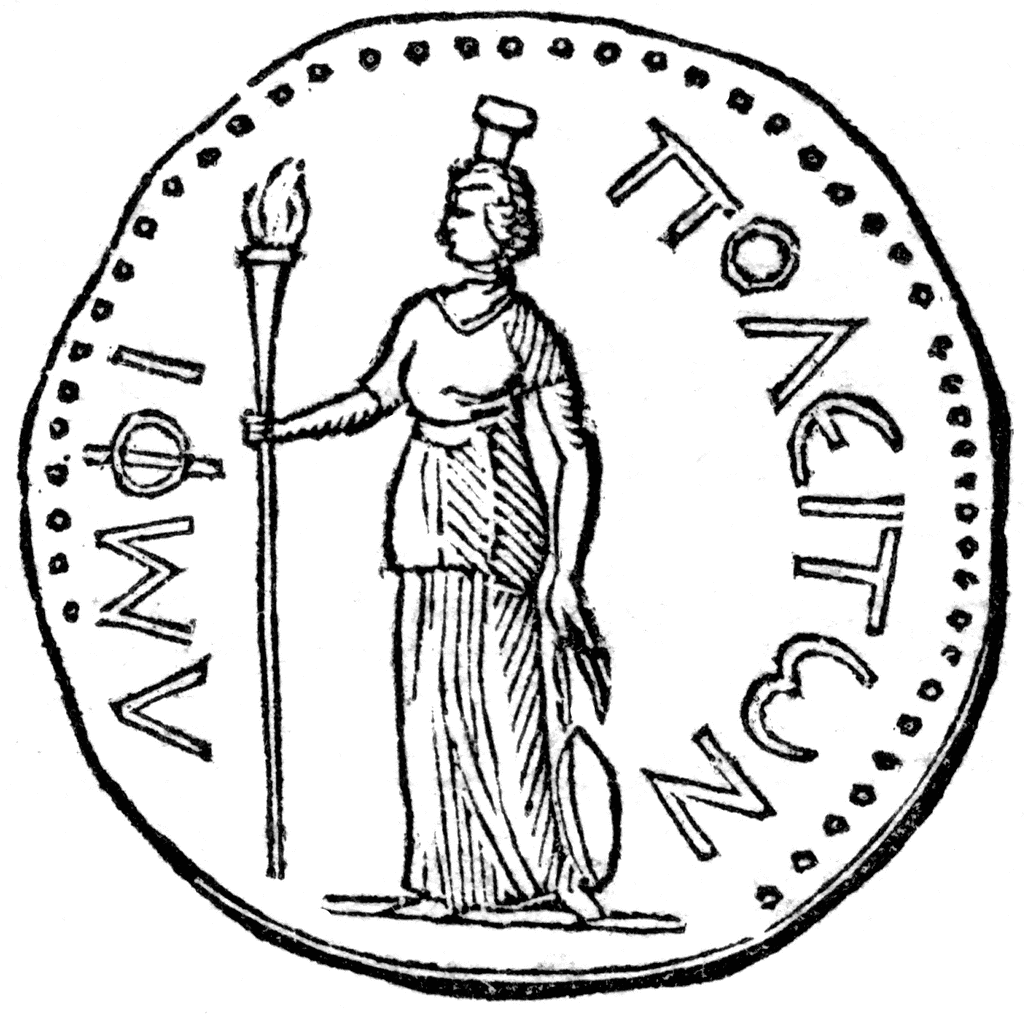
\includegraphics[width=1cm]{TIKZ_SZ/Moneda}};
\draw[>=stealth,->,thick] (-.3,-.35)--(-.75,.45);
\draw (-.525,0) node[left]{\small $\pi_1$};
\draw[>=stealth,->,thick] (-.2,-.35)--(.3,.45);
\draw (.05,0) node[right]{\small $\pi_2 = 1-\pi_1$};
\end{scope}
%
\draw (1.25,-2.25) node{(a)};
\draw (8.25,-2.25) node{(b)};
\end{tikzpicture}